\section{Passivity-Based Control} \label{section:pssivity}
Initial presentation of passive-decomposition is found in D. Lee et. al 2004. \cite{passive-decomp-mechanical-coord-req}. It decomposes the overall dynamics into shape system addressing the coordination aspect, locked system representing internal dynamics wrt. the holonomic constraints and dynamic couplings between the locked and shape systems.The coupled dynamics can be canceled out without violating passivity. Thus, the coordination aspect (shape system) and the dynamics of the coordinated (locked) system can be decoupled from each other while enforcing passivity. By designing the locked and shape controls to enforce passivity  of their respective systems, the closed-loop system energetic passivity is guaranteed. A brief introduction towards passive-decomposition is given as follows. \\
Consider a group of $m$-mechanical systems such that the $i$-th agent's dynamics evolve on a configuration manifold $\Ma_i$:
	\begin{equation}
	M_i(\textbf{q}_i)\nabla^i_{\textbf{v}_i} \textbf{v}_i = \textbf{T}_i + \textbf{F}_i, \;\;\; i = 1,...,m,
\end{equation}
where the following terms are defined as follows:
\begin{itemize}
	\item $\textbf{T}_i, \textbf{F}_i\in\text{T}_{\textbf{q}_i}^*\Ma_i$ - control and environmental force covectors that exist in a cotangent manifold at point $\textbf{q}_i$
	
	\item $\textbf{v}_i \in \text{T}_i^{*}\Ma_i$ - system velocity at point $\textbf{q}_i$ in the tangent manifold
	
	\item $\nabla^i_{\textbf{v}_i}$ - this symbol represents a covariant derivative operator, the Levi-Civita connection. It provides a well defined method of differentiating vector fields along the ${\textbf{v}_i}$ direction on the tangent bundle $\text{T}\Ma_i$.
	
	\item $M_i(\textbf{q}_i)$ - inertia tensor which maps vectors from tangent space to cotangent space at point $\textbf{q}$, defined as $M:\text{T}_{\textbf{q}}\Ma \mapsto \text{T}_{\textbf{q}}^*\Ma$
\end{itemize}

Furthermore, the supply rate for the m-agent mechanical system is defined as follows.
\begin{equation}
	s_\rho(\textbf{v}_i, \textbf{T}_i) = \langle\textbf{F}_i, \dot{\textbf{q}}_i \rangle + ... + \langle\textbf{F}_m, \dot{\textbf{q}}_m \rangle \, ,
\end{equation}
where $\langle \cdot, \cdot \rangle: \text{T}_{\textbf{q}}^*\Ma \times \text{T}_{\textbf{q}}\Ma  \rightarrow \mathbb{R}$. \\
\noindent For safe and stable interaction an energetic passivity condition where $\exists d\in\mathbb{R}$ such that: 
\begin{equation}
	 \int_{0}^{t}	s_\rho(\textbf{v}_i(\tau), \textbf{T}_i(\tau))d\tau \geq -d^2, \;\forall t\geq 0
\end{equation}
Similar condition is employed to induce controller passivity. \\
Introducing the coordination map $h:\Ma^n \rightarrow \Na^m$ which holds the holonomic constraints, at each point of the configuration manifold $q\in\Ma$, the corresponding tangent space $\text{T}_q\Ma$
is split into two orthogonal vector spaces as follows:
\begin{equation}
	\text{T}_q\Ma = \text{T}_q^\top \Ma \oplus \text{T}_q^{\perp} \Ma
\end{equation}
The tangential and perpendicular spaces are defined respectively:
\begin{gather}
	\text{T}_q^\top\Ma := span \{v \in \text{T}_q\Ma \, \vert \, h_*(v) = 0\}  \\
	\text{T}_q^\perp\Ma := span \{w \in \text{T}_q\Ma \, \vert \, \langle \langle v, w \rangle \rangle, \, \forall v \in \text{T}_q^\top \Ma  \}, 
\end{gather}
where $h_*: \text{T}_q\Ma \rightarrow \text{T}_{h(q)}\Na$ is a push-forward of the coordination map. \\
By applying the orthogonal decomposition to the model dynamics we are able to decouple the shape and locked dynamics, while applying a control law cancel the coupling which essentially sums up the notion of passive-decomposition.

A concrete application of the passive-decomposition concepts on a UAV system can be found in \cite{passive-decomp-quadrotor-with-robotic-manip}. The authors show that the Lagrange dynamics of quadrotor-manipulator systems can be completely decoupled into: the center-of-mass dynamics in E(3), which, similar to the standard quadrotor dynamics, is point-mass dynamics with under-actuation  and  gravity  effect; the  “internal rotational” dynamics  of  the  quadrotor’s  rotation  and  manipulator configuration, which assumes the form of standard Lagrange dynamics  of  robotic manipulator with full-actuation and nogravity effect.  
\begin{figure}[H]
	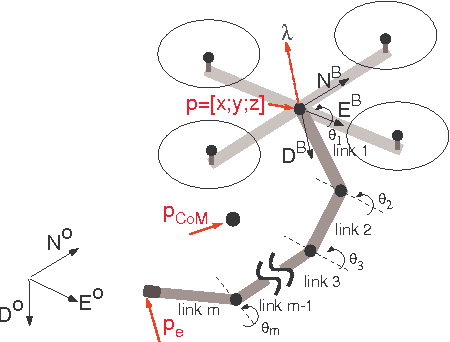
\includegraphics[width=0.95\columnwidth]{figure/aerial_manip.png}	
	\centering
	\caption{This $\text{figure}^{\cite{passive-decomp-quadrotor-with-robotic-manip}}$ represents a quadrotor UAV with a generalized m-DOF robot arm. The UAV platform's position is denoted with $\textbf{p}$, $\textbf{p}_e$ represents the end-effector position while $\textbf{p}_{CoM}$ is the center-of-mass vector of the entire quadrotor-manipulator system. It is worth nothing that a general case is considered where $\textbf{p}_{CoM} \neq\textbf{p}$.  }
	\label{fig:aerial_manip}
\end{figure}
\noindent A backstepping-like end-effector tracking control law is proposed, which allows  assignment of different roles for the center-of-mass control and internal rotational dynamics  control according to task objectives.

A similar passivity-based control design is presented in \cite{decoupled-aerial-manipulation} for quadrotor-manipulator UAV system utilizing a PID cascade  unlike the previously shown backstepping controller. Proposed control algorithms are implemented in the MATLAB/
Simulink environment and tested using the highly nonlinear system model in simulation. 
The controller robustness is checked by applying disturbance forces from different 
directions at the tip point of the 2-DOF robotic arm.

In \cite{passivity-backstepping}  a novel unified passivity-based adaptive backstepping control framework is proposed for ‘mixed’ quadrotor UAVs. It consists of the translation dynamics with thrust force input and the attitude kinematics with the angular velocity input evolving on SE(3). Its application to haptic teleoperation over the Internet is also presented with dynamic-extension like filter to address discontinuous communication and a complete stability/collision-avoidance analysis is provided.

As it was the case with geometric control methods, there are a multitude of applications of passivity-based control on payload carrying and transportation. In \cite{passivity-based-formation-load} the authors propose a strategy consisting of internal feedback control for each UAV and a general formation control law regulating relative positions between each UAV pair. It is proven that under such control strategy the system is stable for all equilibrium points where the cables supporting the suspended load are in tension. \\
\noindent Furthermore, the authors in \cite{passivity-based-payload-minimum-swing} present the Euler-Lagrange formulation quadrotor, cable and payload system. An Interconnection and Damping Assignment-Passivity Based Control (IDA-PBC) for a quadrotor UAV transporting a cable-suspended payload is developed. The designed method does not depend on the swing angle of the cable. Main control objective shown was to transport the payload from point to point, with swing suppression along the desired trajectory. \\ 
It is worth mentioning the research done in \cite{payload-and-human}. A novel concept of master-slave strategy is implemented where the  master  quadrotor  is  controlled  by a human  and  the slave quadrotor tries to stabilize the oscillations of the payload. Two  UAVs with a cable-suspended  payload  is an under-actuated system with coupled dynamics, therefore manual control is proven difficult. A Lyapunov based  controller is designed to  minimize  the  oscillations  of  the  payload while  transportation,  leading  to  an  easier  manual  control  of master quadcopter.

As previously mentioned, one of the main motivations for implementing passive decomposition on UAV systems is to achieve compliant behavior. Research in \cite{passive-variable-impedance-compliant} concerns the notion of passivity-based compliant control methods. The authors introduce a novel scheme, termed Passivity-Preservation Control (PPC), which suppresses the energy injections that could be introduced into compliant robots, as a result of Variable Impedance Control (VIC). Although the presented controller is used with manipulators, this research is still worth mentioning as generally the notion of aerial compliance implies a manipulator endowed UAV. \\
Regarding quadrotors interacting with the environment, in \cite{quadrotor-itneraction-environment} a novel method for applying a wrench while flying is proposed. Inspired by the use of contacts in legged robots, the authors present an idea of exploiting physical contact with the environment, with the goal of going beyond the common thought that the surrounding environment is a constraint to avoid. \\
An energy conservative approach to maximum wrench generation by a fully actuated aerial robot is presented in \cite{max-wrench-min-energy}. Two different approaches for designing the rotor tilt angles of a fully actuated aerial robot are presented in this paper. A common approach is based on maximizing the forces and torques the robot can generate. To determine the tilt angles, simple knowledge of the maximum required wrench is necessary. Another approach focuses on following an a priori defined trajectory with minimum energy consumption, taking advantage of the nonlinear power-thrust characteristic of a real propeller. For this purpose, complex knowledge of the complete trajectory is necessary, especially for rotors with fixed orientation.   \\
A passivity-based control of a fully actuated UAV for aerial physical interaction near hovering is presented in \cite{passivity-based-physical-interaction}. A unified near-hovering motion and impedance controller is derived by the energy-balancing passivity-based control technique. A detailed analysis of the closed-loop system’s behavior  is presented for both the free-flight and contact stability of the UAV. Robustness of the control system to uncertainties is validated by several experiments, in which the UAV is controlled 5near its actuator limits.

\cite{passivity-based-aerial-interaction} \todo[inline]{TODO:}

\begin{figure}[H]
	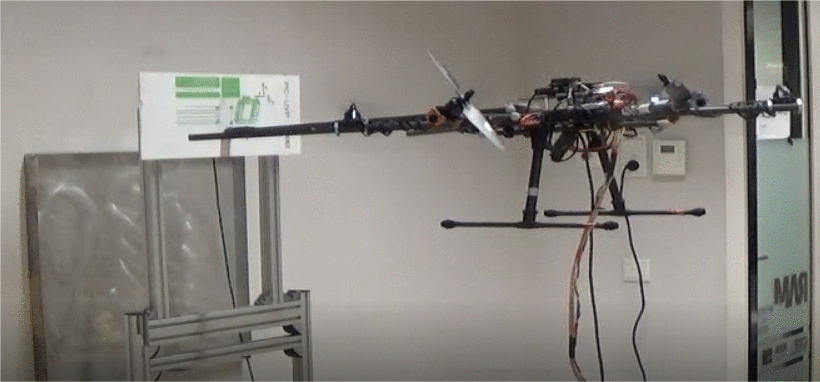
\includegraphics[width=0.95\columnwidth]{figure/passivity-based-interaction.png}	
	\centering
	\caption{This $\text{figure}^{\cite{passivity-based-physical-interaction}}$ represents a fully-actuated hexarotor UAV hovering with one rotor off and applying ~10N of force to a verticl surface rigidly connected to a force sensor.}
	\label{fig:aerial_compliance}
\end{figure}

\cite{door-opening}

\todo[inline]{TODO: cite all inspection methods} 
 \cite{ref:corosion-inspection}\cite{ref:inspection-overview}\cite{Ollero2018} \cite{ref:sar}  \cite{ref:lidar-equipped-model-building}

\cite{passivity-based-crop} 
\cite{cooperative-control-quadrotor}
\cite{haptic-teleoperation-uav}